\chapter{海量数据分析与车辆移动模型建立}

<建模规则概述>

\section{出租车数据介绍}
从“北京智能交通系统关键技术研究与应用示范项目”获取的数据集,该项目以支持智能交通系统工程建设、解决关键技术难题、提升交通科技发展水平和自主创新能力、为实现新北京交通体系和奥运会的顺利召开提供支持与保障为目标。其核心研发内容之一,是实时采集、存储、处理多源异构海量交通数据、形成动态交通信息以及决策支持的分布式处理系统。该项目涉及出租车为12096辆,约占北京市出租车总数的$18\%$,对五环内(含五环)次干路以上路网的覆盖率达到$90\%$以上。通过这些出租车上安装的GPS定位装置,每隔约60s上传一次自己的经纬度位置、速度、方向信息到数据中心。每天产生的数据量约1300万条。
数据记录格式如表\ref{table_dataset}所示。

\begin{table}
\caption{北京市出租车数据格式和字段意义}\label{table_dataset}
\begin{tabular}{l|c}
\hline
列名&	说明\\
\hline
调度中心ID&	4个ASCII字符;\\
\hline
出租公司ID&	标记出租车为何公司所有.\\
\hline
车辆ID&	使用11个ASCII字符;\\
\hline
时间标签&	使用GMT时间格式共14个ASCII字符,格式为(YYYYMMDDHHMMSS);\\
\hline
84坐标系经度&	最长为11个ASCII字符,变长;\\
\hline
84坐标系纬度&	最长为10个ASCII字符,变长;\\
\hline
02坐标系经度&	一般为9个ASCII字符,除以3686400(1024*3600)后变为通用经度坐标;\\
\hline
02坐标系纬度&	一般为9个ASCII字符,除以3686400(1024*3600)后变为通用纬度坐标;\\
\hline
速度&	单位为公里/小时,最长为3个ASCII字符,变长;\\
\hline
方向&	以正北为0度,顺时针方向增大,为0~360角度,最长为3个ASCII字符,变长;\\
\hline
状态&	为1个ASCII字符,数值型字符,包括空载、满载等状态。\\
\hline
事件(event)&	为1个ASCII字符,数值型字符,包括上下车、开锁车门等。\\
\hline
高度&	两个ASCII字符,固定值为50,未使用\\
\hline
\end{tabular}
\end{table}



\section{出租车行为假设}

在日常生活中,我们打车可能需要走到小区或者学校门口,在车站,飞机厂等地也都设有专门的打车区域,基于我们日常生活经验和主观感受,我们提出了以下假设:
%假设1
\begin{assumption}\label{assuption_1}
\textbf{车辆行为与其车辆状态有关。}当一辆出租车处于载客状态时,它的目的地是确定的,其速度会相对增加。相反的,当一辆出租车处于空载状态时,出租车可能会减速甚至停靠在路边来寻找或等待可能的客人。这样,出租车的行为,例如车辆速度和状态持续时间都会随着车辆状态的变化而变化。
\end{assumption}
%假设2
\begin{assumption}\label{assuption_2}
\textbf{车辆的行为与其时间因素有关。}
车辆在不同时间段的上下客的数量可能与时间服从一定的规则。例如,晚上的客人数量会相对于白天的客人有所减少。其与时间的相关性还有可能体现在以下几个方面。
\begin{itemize}
\item 上下客的热点区域可能会随着时间变化而发生变化。
\item 上下课的事件数可能会随着时间的变化而变化。例如凌晨发生载客和下客事件的数量都会相对减少,而到了白天,去往商场,写字楼等热门区域的出租车载客和下客的数量都会明显增多。
\end{itemize}
\end{assumption}
%假设3
\begin{assumption}\label{assuption_3}
\textbf{车辆行为与其地理因素有关。}
当一辆出租车处于载客状态时,出租车的目的地更可能是某些特定区域,例如机场,火车站等。同时,当出租车为空载状态时,出租车更倾向于选择附近的热点区域,在这样的区域内,人们更倾向于打车,例如某些商业街,电影院。车辆行为与地理因素的相关性可能体现在以下方面:
\begin{itemize}
\item 出租车选择目的地点与出租车的当前位置有关。
\item 事件在不同区域发生的概率不同。
\item 不同事件在相同区域发生的概率不同。
\end{itemize}
\end{assumption}

接下来,为了验证我们的假设,我们基于北京市出租车数据对车辆的速度,状态持续时间,

\section{海量数据分析}
\subsection{出租车不同状态速度和持续时长分析}

\begin{figure}[ht]
\centering
\begin{tabular}
[c]{c}
\epsfysize=2in\epsfbox{figures/analysis/avgsp_vacant.eps} \\
(a) vacant status \\ 
\epsfysize=2in\epsfbox{figures/analysis/avgsp_occupied.eps} \\
(b) occupied status \\
\end{tabular}
\caption{空载和载客状态下每小时的平均速度}\label{figure_avg_speed}
\end{figure}
\begin{figure}[ht]
\centering
\begin{tabular}
[c]{cc}
\epsfysize=1.5in\epsfbox{figures/analysis/speed6_0.eps} &
\epsfysize=1.5in\epsfbox{figures/analysis/speed6_1.eps} \\ 
\multicolumn{2}{c}{6:00-8:00}\\
\epsfysize=1.5in\epsfbox{figures/analysis/speed11_0.eps} &
\epsfysize=1.5in\epsfbox{figures/analysis/speed11_1.eps}\\
\multicolumn{2}{c}{11:00-13:00}\\
\epsfysize=1.5in\epsfbox{figures/analysis/speed17_0.eps} &
\epsfysize=1.5in\epsfbox{figures/analysis/speed17_1.eps}\\
\multicolumn{2}{c}{17:00-19:00}\\
\epsfysize=1.5in\epsfbox{figures/analysis/speed22_0.eps} &
\epsfysize=1.5in\epsfbox{figures/analysis/speed22_1.eps}\\
\multicolumn{2}{c}{22:00-24:00}\\
(a) vacant status& (b) occupied status\\
\end{tabular}
\caption{不同时间段,空载和载客状态下的速度分布情况}\label{figure_speed_distribution}
\end{figure}

\begin{figure}[ht]
\centering
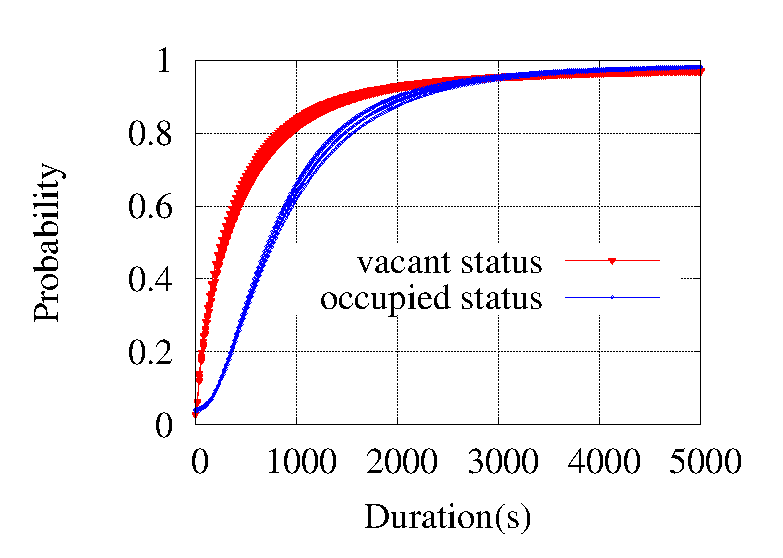
\includegraphics[width=0.5\textwidth]{figures/assumption/durationdis.eps}\\
\caption{状态持续时长分布}\label{figure_duration_for_each_status}
\end{figure}


\subsection{随时间变化的事件分布}


\begin{figure}[ht]
\centering
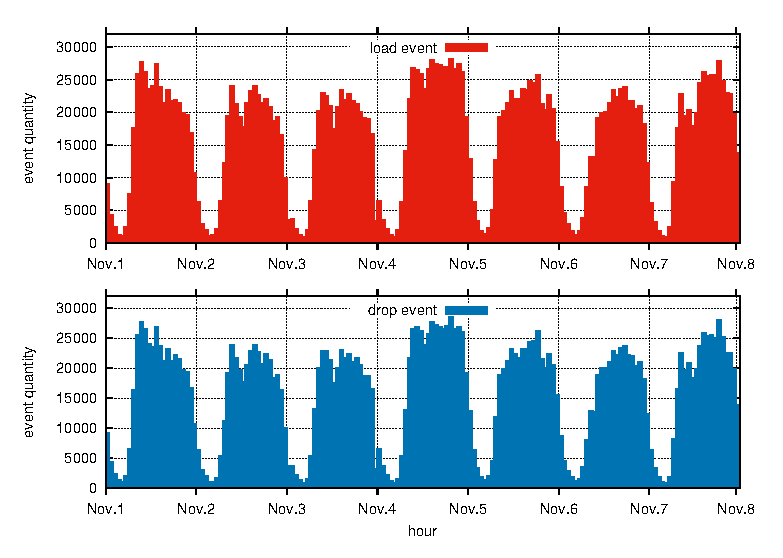
\includegraphics[width=0.65\textwidth]{figures/analysis/event_w_time.eps}\\
\caption{Taxi event varied with time.}\label{figure_event_varied_w_t}
\end{figure}



\begin{table}[ht]
\caption{随时间变化的事件数}\label{table_event_distribution_with_time}
\centering
\begin{tabular}{l|c|c}
 \hline
 名称 & 下客事件数 & 上客事件数 \\
  \hline
  一周总数& 2,679,385&2,707,290\\
  一小时内最大值&28,583 &28,130\\
  一小时内最小值&861&918\\
  波峰时段&11月4日, 19:00-20:00&11月4日, 19:00-20:00\\
  波谷时段&11月3日, 4:00-5:00&11月3日, 4:00-5:00\\
  \hline
  \end{tabular}
\end{table}




\begin{figure}[ht]
\centering
\fbox{\includegraphics[width=0.4\textwidth]{figures/map.eps}}\\
\caption{抽取地图}\label{figure_map}
\end{figure}


\begin{figure}[ht]
\centering
\begin{tabular}
[c]{cc}
\epsfysize=2in\epsfbox{figures/analysis/hotspots/hotspot_drop_04.eps} &
\epsfysize=2in\epsfbox{figures/analysis/hotspots/hotspot_drop_19.eps} \\
(a) drop events at 4:00-5:00 & (b) drop events at 19:00-20:00\\
\epsfysize=2in\epsfbox{figures/analysis/hotspots/hotspot_load_04.eps} &
\epsfysize=2in\epsfbox{figures/analysis/hotspots/hotspot_load_19.eps} \\
(c) load events at 4:00-5:00 & (d) load events at 19:00-20:00\\
\end{tabular}
\caption{Taxi density for load/drop events in one hour.}\label{figure_taxi_density_for_one_hour}
\end{figure}


\begin{figure}[ht]
\centering
\begin{tabular}
[c]{cccc}
\epsfysize=1in\epsfbox{figures/analysis/hotspots/1hotspot_20_drop_19.eps} &
\epsfysize=1in\epsfbox{figures/analysis/hotspots/3hotspot_20_drop_19.eps} &
\epsfysize=1in\epsfbox{figures/analysis/hotspots/5hotspot_20_drop_19.eps} &
\epsfysize=1in\epsfbox{figures/analysis/hotspots/6hotspot_20_drop_19.eps} \\
(a) 11月1日,周二 &(b) 11月3日, 周四 &(c) 11月5日, 周六 &(d) 11月6日,周日 \\
\multicolumn{4}{c}{下客事件热点区域}\\
\epsfysize=1in\epsfbox{figures/analysis/hotspots/1hotspot_20_load_19.eps} & 
\epsfysize=1in\epsfbox{figures/analysis/hotspots/3hotspot_20_load_19.eps} &
\epsfysize=1in\epsfbox{figures/analysis/hotspots/5hotspot_20_load_19.eps} &
\epsfysize=1in\epsfbox{figures/analysis/hotspots/6hotspot_20_load_19.eps} \\
(e) 11月1日,周二 &(f) 11月3日, 周四 &(g) 11月5日, 周六 &(h) 11月6日,周日 \\
\multicolumn{4}{c}{载客事件热点区域}\\
\end{tabular}
\caption{出租车一小时内载客和下客事件的数量的区域分布}\label{figure_taxi_density_for_one_hour}
\end{figure}


\section{建立模型}

移动模型定义了节点的运动模式$Paths:<p_1,p_2…,p_n>$,$p_i$的确定可以简化为两步,即,目的地点选择和从源地点到目的地点的移动模式。
目的地点选择:节点的目的选择也与节点的当前状态有关。若节点处于载客状态。若当前状态为载客状态:针对载客事件将区域划分为不同的子区域,同理由下客事件分布将区域划分为不同的子区域。计算由载客子区域到下客子区域的转移概率矩阵和距离范围。然后由节点当前位置,决定下客位置。同理,节点处于下客状态时,由当前位置,和区域转移矩阵也可以计算得到载客的目的节点。


\subsection{区域定义与识别}

如何划分和识别区域是当前研究中的一个难点,也是计算区域转移矩阵的基础。现有研究中的区域识别有简单的讲区域划分为$n\times m$的网格,这种情况下当网格的粒度变大,其计算复杂度也急剧上升。对于$n\times m$的网格来说,其计算区域转移矩阵的复杂度为$O(n^2 \times m^2)$。另一种常用方式是通过手动的划分,对区域的按照某个属性(例如小区)划分。这种划分方式对于特定情境较为符合,但是可扩展性不强,且带有较大的主观性。
因此为了保证区域转移概率的准确度,计算效率以及可扩展性,我们采用了讲区域划分为细粒度的网格后再进行聚类。

此外我们区域按照不同时段以及不同的事件类型动态划分。
首先,我们
\begin{definition}
\label{cell}
\textbf{格子为区域识别中的最小单位,规定某块区域的范围,也表示一段连续经纬度的集合。}本文将之定义为矩形格子。记为:
\begin{equation}
C_{x,y}::=\{(lon,lat)|x \le \frac{{lon}}{{X}} < x + 1,
y \le \frac{{lat}}{{Y}} < y + 1\}.
\end{equation}
\end{definition}


其中,$C_{x,y}$ 表示编号为$(x,y)$的格子,$lon$ 和 $lat$ 表示经度和纬度,$X$和$Y$表示经度和纬度方向上每个格子的长度。基于格子可以定义区域。

\begin{definition}
\label{def_region}
\textbf{区域是一些连续格子的集合,在本文中,也是区域转移概率矩阵计算的最小单位。}记为:

\begin{equation}
R_m:: = \{ C_{i,j}|if C_{x,y} \in R_m
\Rightarrow \|x - i\| \le 1,\|y - j\| \le 1\}.
\end{equation}

\end{definition}

我们按照对应时间段对应事件发生的事件数对之进行划分。由于事件分布及其不均匀,我们同时也规定了两种区域,一种是事件密集区域,一种是事件稀疏区域。当区域中的每个格子的事件数均大于阈值$\eta$时,该区域为密集区域,否则为稀疏区域。事件密集区域为$\_top$个,为了减少密集区域仅包含一个或少数几个格子。同时为了保证区域大小不至于过大,我们定义了一个区域最多包含$ClusterSize$个格子,即$\|R_i\|\leq ClusterSize$。

对于某个时段的某一事件类别,我们首先计算每个格子发生的该类别事件数。首先需要找出$\_top$个密集区域,我们先降序排序,从事件最密集的格子开始,进行广度遍历,如果事件数大于$\eta$,则加入区域中,每个格子属于且仅属于一个区域。找到$\_top$个区域后,我们剩下的格子内的事件数不需要大于$_eta$,仅需要满足$\|R_i\|\leq ClusterSize$.

$\eta$设为整个场景中应时间段和事件类型的事件数的均值的两倍,区域识别的相关参数如下表\ref{table_region_rec},区域识别的具体算法见附录.


\begin{table}
\caption{区域识别相关参数}\label{table_region_rec}
\centering
\begin{tabular}{l|c|c|c|c}
  \hline
  Item & 0:00-8:59 &9:00-12:59&13:00-20:59 &21:00-23:59 \\
  \hline
  $\eta_{drop}$ & 56&84 &180 &51\\
  $\eta_{load}$ & 58&84 &182 &51\\
  \_top & 200&200 &200 &200\\
  clusterSize& 500&500 &500 &500\\
  \hline
\end{tabular}
\end{table}


\begin{figure}[ht]
\centering
\subfigure[drop event regions]{\includegraphics[width=0.33\textwidth]{figures/region/Areas-2011_event01.eps}}
\subfigure[load event regions]{\includegraphics[width=0.33\textwidth]{figures/region/Areas-2011_event03.eps}}
\centering
\caption{Region recognition}\label{figure_region_recognizition}
\end{figure}

区域识别的结果如图\ref{figure_region_recognizition},其中每个色块都代表一个区域,由图可知,北京市的事件分布主要集中在主干道路上,其他较为规则的区域为稀疏区域,主要分布在城市周边。




\subsection{区域转移概率}
区域转移概率


\subsection{时间建模}
\input{cpts/sects/model-time}

\subsection{速度建模}
\begin{figure}[!h]
\centering
\begin{tabular}
[c]{cc}
\multicolumn{2}{c}{6:00-8:00}\\
\epsfysize=1.5in\epsfbox{figures/evalue/fitspeed6_0.eps} &
\epsfysize=1.5in\epsfbox{figures/evalue/fitspeed6_1.eps} \\
\multicolumn{2}{c}{11:00-13:00}\\
\epsfysize=1.5in\epsfbox{figures/evalue/fitspeed11_0.eps} &
\epsfysize=1.5in\epsfbox{figures/evalue/fitspeed11_1.eps} \\
\multicolumn{2}{c}{17:00-19:00}\\
\epsfysize=1.5in\epsfbox{figures/evalue/fitspeed17_0.eps} &
\epsfysize=1.5in\epsfbox{figures/evalue/fitspeed17_1.eps} \\
\multicolumn{2}{c}{22:00-24:00}\\
\epsfysize=1.5in\epsfbox{figures/evalue/fitspeed22_0.eps} &
\epsfysize=1.5in\epsfbox{figures/evalue/fitspeed22_1.eps} \\
(a) vacant status & (b) occupied status \\
\end{tabular}
\caption{速度分布的拟合结果}\label{figure_fitspeed_varied_with_time}
\end{figure}



为了获取各个状态的速度分布,我们对瞬时速度的累积分布进行拟合,以获取瞬时速度的累积分布函数,然后衍生出其速度分布函数。
由图\ref{figure_fitspeed_varied_with_time}可知,除了载客状态时从22:00-24:00的累积瞬时速度分布外,瞬时速度的累积分布表现出指数分布的规律,拟合函数记为$f_1(x)$。载客状态时从22:00-24:00的累积瞬时速度分布表现出线性分布的特性,其拟合函数记为$f_2(x)$, 如公式\ref{formular_ccdf_speed}。由分析过程可知,某些天,例如周末的某些时段会影响车辆的行为,我们仅分析最常见的情况,因此去掉了明显不一样的情况,例如周六和周天早上6点到8点时的载客状态的累积速度分布。

\begin{equation}\label{formular_ccdf_speed}
\left\{
\begin{array}{ll}
f_1(x) = 1-1/exp(-ax^b-c)\\
f_2(x) = ax+b
\end{array}
\right.
\end{equation}

\begin{table}[ht]
\caption{拟合参数以及拟合曲线的残差平方和}\label{table_rms}
\centering
\begin{tabular}{c|c|c}
  \hline
  时间段 & 空车状态 & 载客状态 \\
  \hline
6:00-8:00   &0.0129207 & 0.019818 \\
11:00-13:00 &0.00866176 & 0.0204889 \\
17:00-19:00 &0.0176578 & 0.0105868 \\
22:00-24:00 &0.0154822 & 0.0240426 \\
  \hline
\end{tabular}
\end{table}

拟合结果以及相关的残差平方和(root mean square, rms)如表\ref{table_rms}所示,越小的残差平方和代表越小的误差。由表\ref{table_rms}可知,所有的残差平方和均小于$0.025$,表现出较好的拟合相似性。


\section{本章小结}
本章详细描述了整体的建立出租车移动模型思路,移动模型的思路可以简化为多次移动的过程,对于每一次移动,都可以分为目的点的选区及其从原点到目的点的移动过程。其中目的点的选取由区域转移概率矩阵计算得出,而移动过程采用了最短路径算法并对其移动的速度建模。本章针对其中的关键点,包括地图抽取,区域识别,区域转移概率的计算以及速度建模进行了详细的说明,并给出了特定条件下的拟合结果和误差。
